\subsubsection{Pengumpulan Data}

Tahap pengumpulan data dilakukan untuk memperoleh citra Nasi Padang yang akan digunakan dalam proses pelatihan dan pengujian model YOLO11-seg. Data yang dikumpulkan berupa citra piring Nasi Padang yang memuat satu atau lebih lauk dari kelas yang digunakan dalam penelitian.

Pengumpulan citra dilakukan melalui dua sumber, yaitu pengambilan citra secara langsung dan pengumpulan citra dari internet. Pengambilan citra secara langsung dilakukan untuk memperoleh citra yang sesuai dengan kondisi penggunaan sistem, sedangkan citra dari internet digunakan untuk menambah variasi tampilan lauk, seperti bentuk, penyajian, posisi objek, dan kondisi pencahayaan.

Citra yang dikumpulkan kemudian melalui proses seleksi sebelum digunakan sebagai dataset. Citra yang tidak menampilkan objek dengan cukup jelas, memiliki kualitas yang terlalu rendah, merupakan duplikat, atau memiliki elemen visual yang menutupi sebagian besar objek tidak digunakan. Seleksi tersebut dilakukan agar citra yang digunakan tetap memberikan informasi visual yang memadai untuk proses anotasi dan pelatihan model.

Dataset difokuskan pada sembilan kelas yang digunakan dalam sistem, yaitu nasi, rendang, ayam goreng, perkedel, sayur nangka, daun singkong, telur dadar, telur kari, dan sambal. Satu citra dapat mengandung lebih dari satu kelas maupun lebih dari satu instans dari kelas yang sama. Kondisi tersebut diperlukan karena pada penggunaan sistem, satu piring dapat berisi beberapa jenis lauk secara bersamaan.

Selain citra dengan objek yang terlihat secara terpisah, dataset juga dapat memuat citra dengan kondisi objek saling bersentuhan atau mengalami oklusi. Kondisi oklusi tidak diasumsikan dapat diselesaikan sepenuhnya oleh model, tetapi digunakan sebagai salah satu kondisi yang akan dievaluasi untuk mengetahui perubahan performa YOLO11-seg dibandingkan dengan kondisi non-oklusi.

Citra yang telah lolos proses seleksi selanjutnya digunakan pada tahap anotasi. Setiap objek yang termasuk dalam sembilan kelas penelitian akan diberikan anotasi kelas dan area segmentasi sehingga dapat digunakan sebagai \textit{ground truth} dalam proses pelatihan YOLO11-seg.

Contoh citra yang digunakan dalam dataset ditunjukkan pada Gambar~\ref{fig:contoh-dataset}.

\begin{figure}[H]
    \centering
    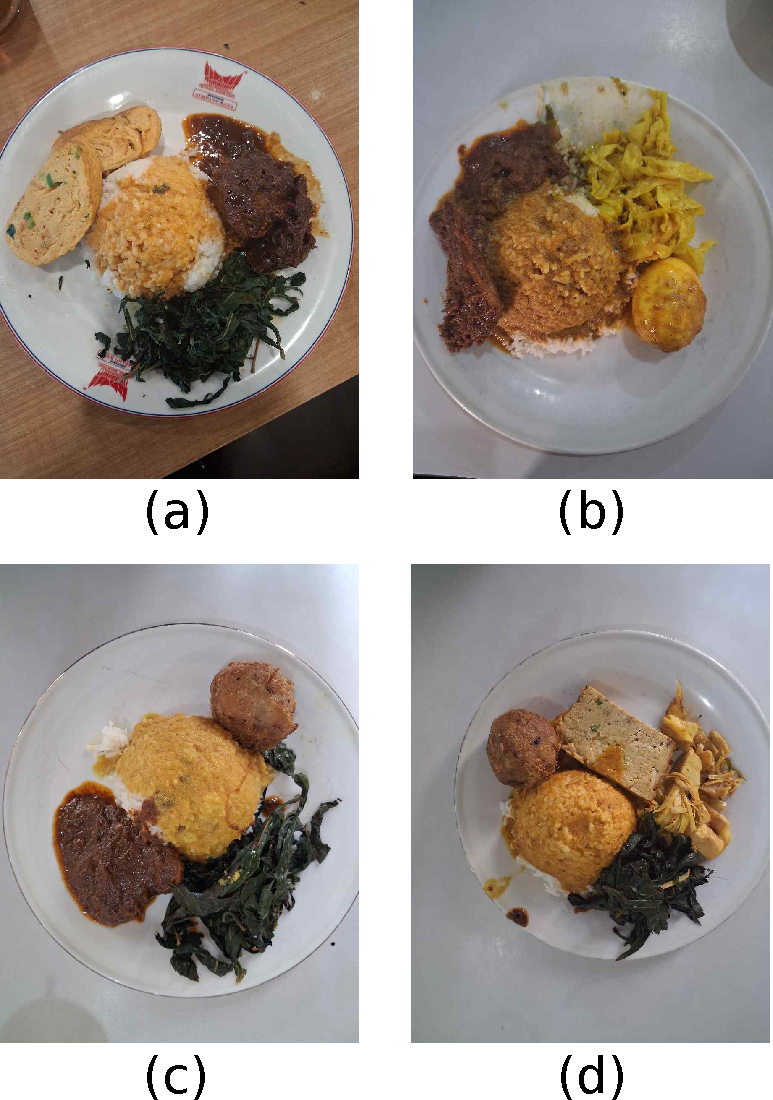
\includegraphics[width=0.55\textwidth]{figures/contoh_dataset.pdf}
		\caption{Contoh citra hasil pengumpulan data secara langsung}
    \label{fig:contoh-dataset}
\end{figure}
